\documentclass{beamer}

\usetheme{Copenhagen}
\usecolortheme{orchid}
\title{CacaoScript: Syntax and Semantics}
\subtitle{A simple language for distributed applications on CacaoWeb}
\author{Ivan Chollet,Lucius Gregory Meredith,Paul Steckler}
\date{\today}

\newcommand{\ldb}{[\![}
%\newcommand{\ldb}{\lefthalfcup}
\newcommand{\rdb}{]\!]}
%\newcommand{\rdb}{\righthalfcup}
\newcommand{\meaningof}[1]{\ldb #1 \rdb}
%\newcommand{\meaningof}[1]{\lefthalfcup #1 \righthalfcup}

\AtBeginSection[]
{
  \begin{frame}
    \frametitle{ToC}
    \tableofcontents[currentsection]
  \end{frame}
}

\begin{document}
  \frame{\titlepage}
  \section{Overview}
  \section{Syntax}
  \begin{frame}
    \frametitle{Syntax}
    \begin{itemize}
      \item Core language is a mini-OCaml
      \item with sugar for
        \begin{itemize}
          \item Comprehensions
          \item Delimited continuations
          \item Reflection (quote and unquote)
        \end{itemize}
    \end{itemize}
  \end{frame}
  \subsection{Core language}
  \begin{frame}
    \frametitle{Core language I}
    \begin{figure}[ht]
      \begin{center}        
        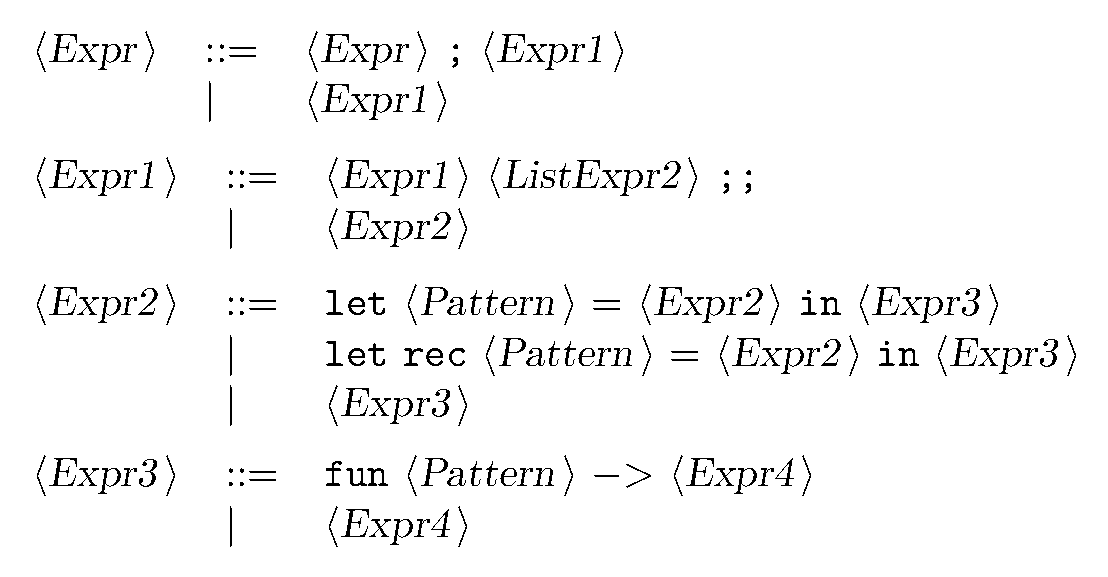
\includegraphics[height=2in]{pipelinefigures/CoreLanguageSyntaxI.pdf}
      \end{center}      
    \end{figure}
  \end{frame}
  \begin{frame}
    \frametitle{Core language II}
    \begin{figure}[ht]
      \begin{center}        
        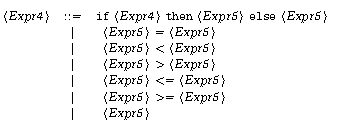
\includegraphics[width=\textwidth,height=0.8\textheight,keepaspectratio]{pipelinefigures/CoreLanguageSyntaxII.pdf}
      \end{center}      
    \end{figure}
  \end{frame}
  \begin{frame}
    \frametitle{Core language III}
    \begin{figure}[ht]
      \begin{center}        
        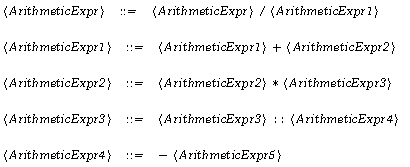
\includegraphics[width=\textwidth,height=0.8\textheight,keepaspectratio]{pipelinefigures/CoreLanguageSyntaxIII.pdf}
      \end{center}      
    \end{figure}
  \end{frame}
  \subsection{Sugar}
  \subsubsection{Comprehensions}
  \begin{frame}
    \frametitle{Comprehensions}
    \begin{figure}[ht]
      \begin{center}        
        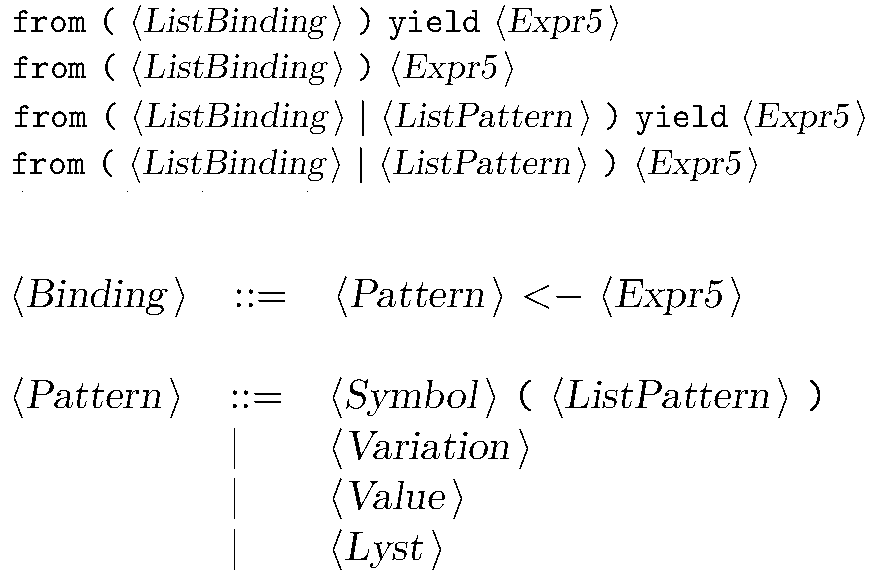
\includegraphics[height=2in]{pipelinefigures/SyntaxSugarComprehensions.pdf}
      \end{center}      
    \end{figure}
  \end{frame}
  \subsubsection{Delimited continuations}
  \begin{frame}
    \frametitle{Delimited continuations}
    \begin{figure}[ht]
      \begin{center}        
        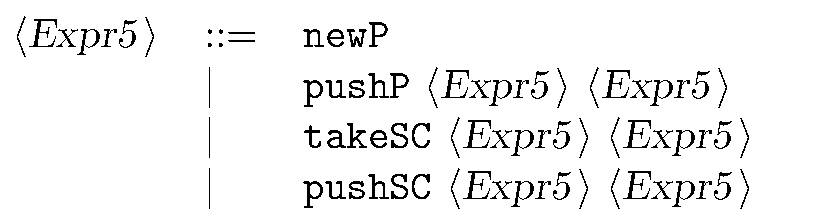
\includegraphics[width=\textwidth,height=0.3\textheight,keepaspectratio]{pipelinefigures/SyntaxSugarDelimCC.pdf}
      \end{center}      
    \end{figure}
  \end{frame}
  \subsubsection{Reflection}
  \begin{frame}
    \frametitle{Reflection}
  \end{frame}
  \section{Example programs}
  \begin{frame}
    \frametitle{Example programs}
    \begin{itemize}
      \item simple arithmetic
      \item obligatory lambda abstraction application example
      \item in-place update of a key-value map
      \item concurrency examples        
    \end{itemize}
  \end{frame}
  \subsection{The basics: arithmetic}
  \begin{frame}
    \frametitle{Sum, products, etc}    
    We can write down any continued fraction such as
    $P/Q = a + 1/(b + 1/(c + 1/(d + \ldots)))$        
    \begin{figure}[ht]
      \begin{center}        
        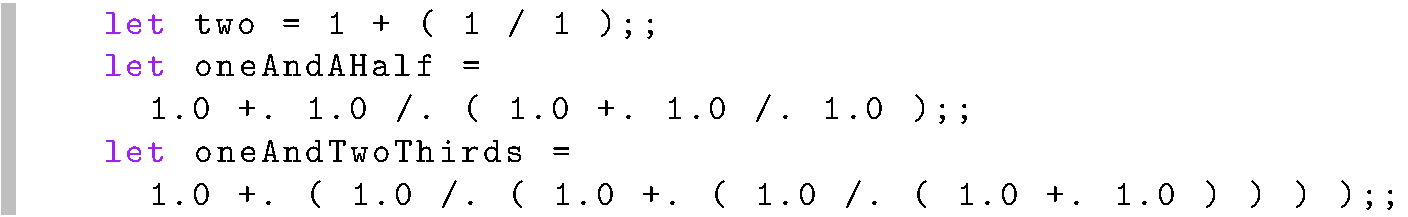
\includegraphics[width=\textwidth,height=0.8\textheight,keepaspectratio]{pipelinefigures/CodeSamplesArithmetic.pdf}
      \end{center}      
    \end{figure}
%     let two = 1 + ( 1 / 1 );;
%     let oneAndAHalf = 1.0 +. 1.0 /. ( 1.0 +. 1.0 /. 1.0 );;
%     let oneAndTwoThirds = 1.0 +. ( 1.0 /. ( 1.0 +. ( 1.0 /. ( 1.0 +. 1.0 ) ) ) );;
  \end{frame}
  \subsection{The basics: abstraction and application}
  \begin{frame}
    \frametitle{$(\lambda x.x)(\lambda x.x)$}    
    \begin{figure}[ht]
      \begin{center}        
        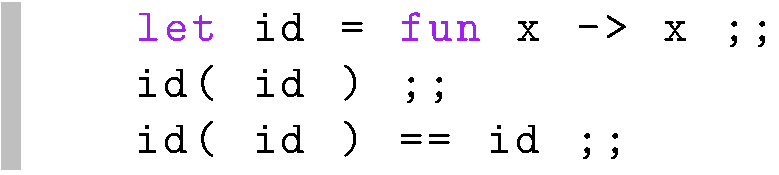
\includegraphics[width=\textwidth,height=0.2\textheight,keepaspectratio]{pipelinefigures/CodeSamplesAbstractionApplication.pdf}
      \end{center}      
    \end{figure}
%     let id = fun x -> x ;;
%     id( id ) ;;
%     id( id ) == id ;;
  \end{frame}
  \subsection{More realistic examples}
  \begin{frame}
    \frametitle{Continued fractions}    
    \begin{figure}[ht]
      \begin{center}        
        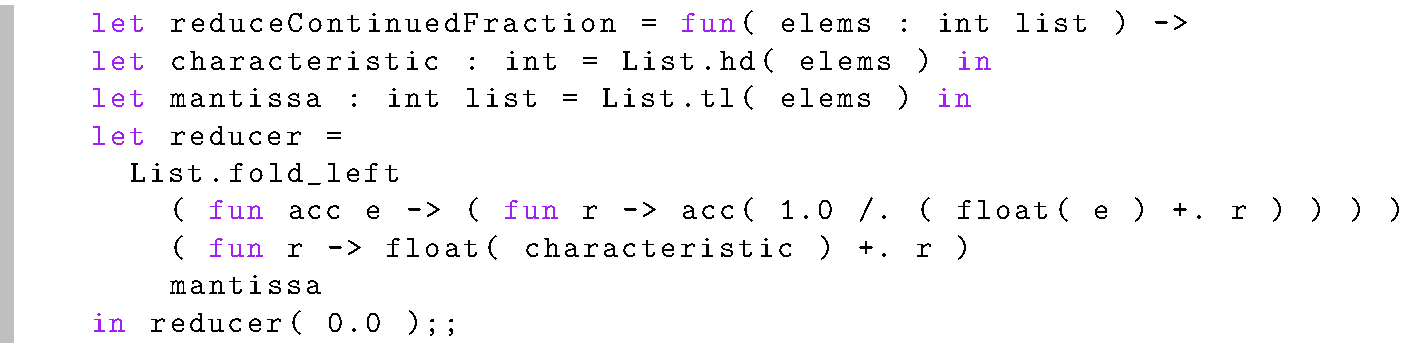
\includegraphics[width=\textwidth,height=0.8\textheight,keepaspectratio]{pipelinefigures/CodeSampleContinuedFractions.pdf}
      \end{center}      
    \end{figure}
  \end{frame}
  \begin{frame}
    \frametitle{in-place update with delimcc}    
    \begin{figure}[ht]
      \begin{center}        
        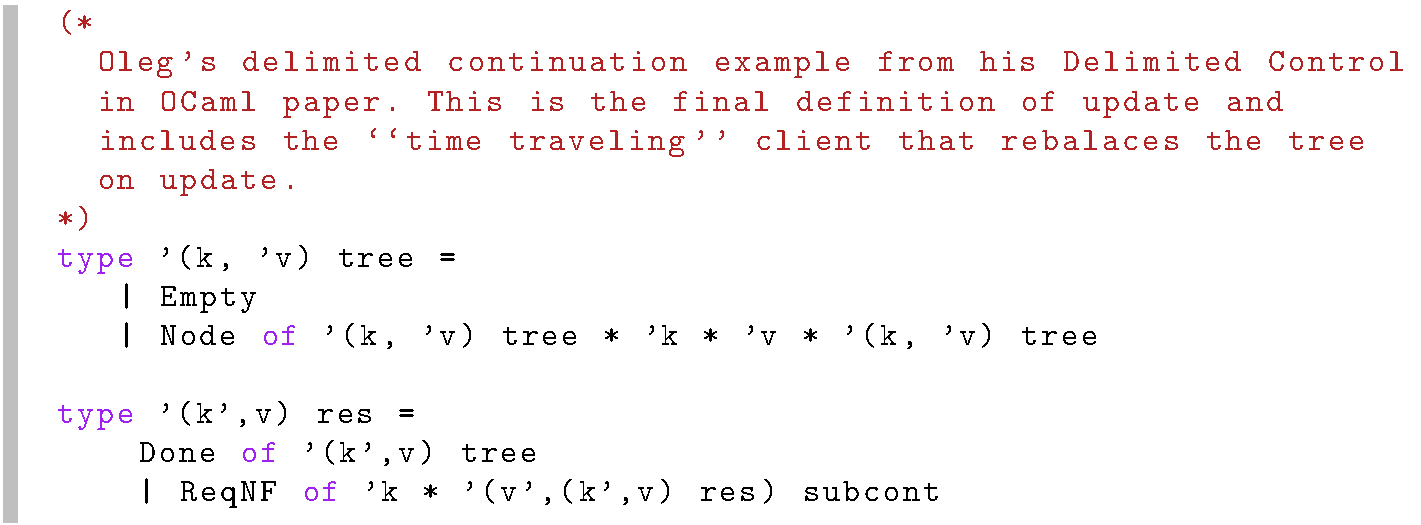
\includegraphics[width=\textwidth,height=0.8\textheight,keepaspectratio]{pipelinefigures/CodeSamplesDelimCCInplaceUpdateTypes.pdf}
      \end{center}      
    \end{figure}
  \end{frame}
  \begin{frame}
    \frametitle{in-place update with delimcc}    
    \begin{figure}[ht]
      \begin{center}        
        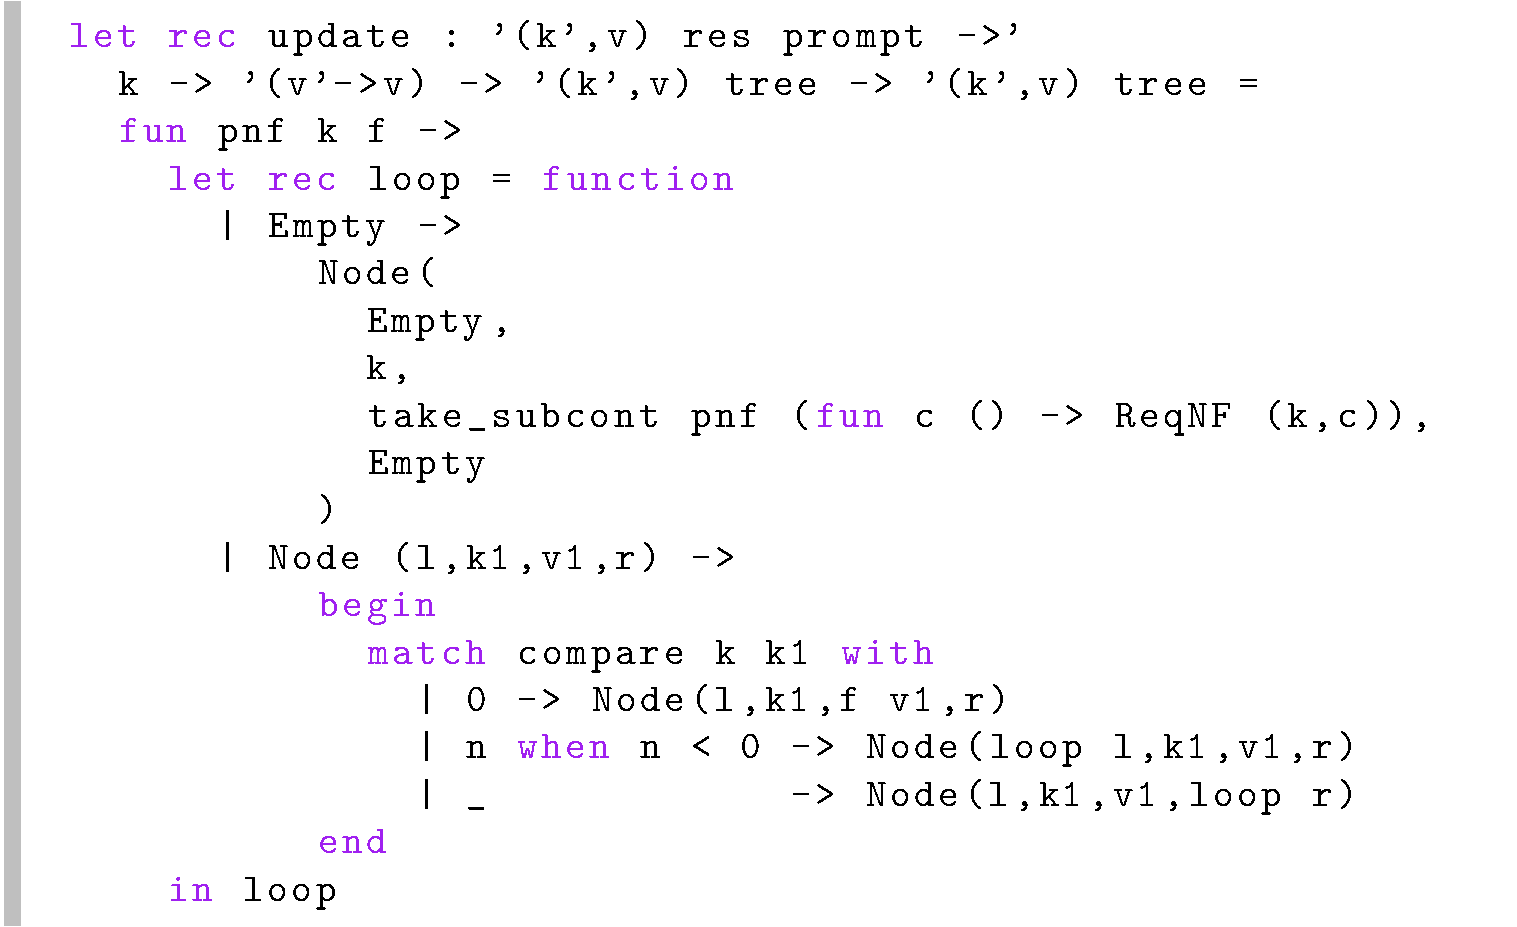
\includegraphics[width=\textwidth,height=0.8\textheight,keepaspectratio]{pipelinefigures/CodeSamplesDelimCCInplaceUpdateTraversal.pdf}
      \end{center}      
    \end{figure}
  \end{frame}
  \begin{frame}
    \frametitle{in-place update with delimcc}    
    \begin{figure}[ht]
      \begin{center}        
        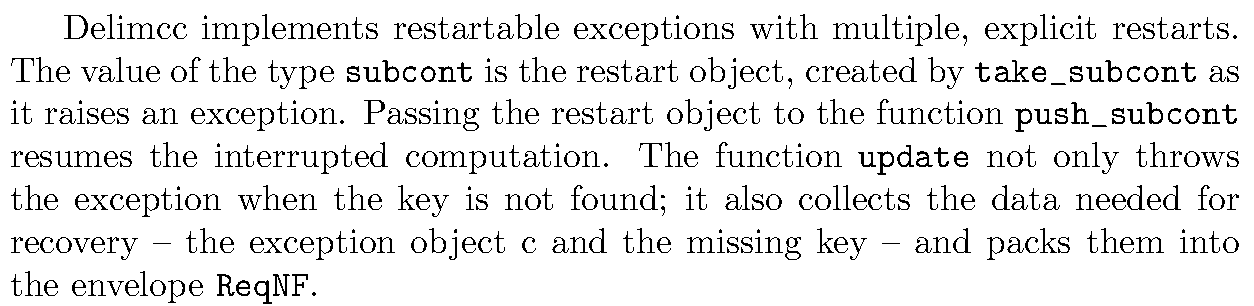
\includegraphics[width=\textwidth,height=0.8\textheight,keepaspectratio]{pipelinefigures/CodeSamplesDelimCCExplanationI.pdf}
      \end{center}      
    \end{figure}
  \end{frame}
  \begin{frame}
    \frametitle{in-place update with delimcc}    
    \begin{figure}[ht]
      \begin{center}        
        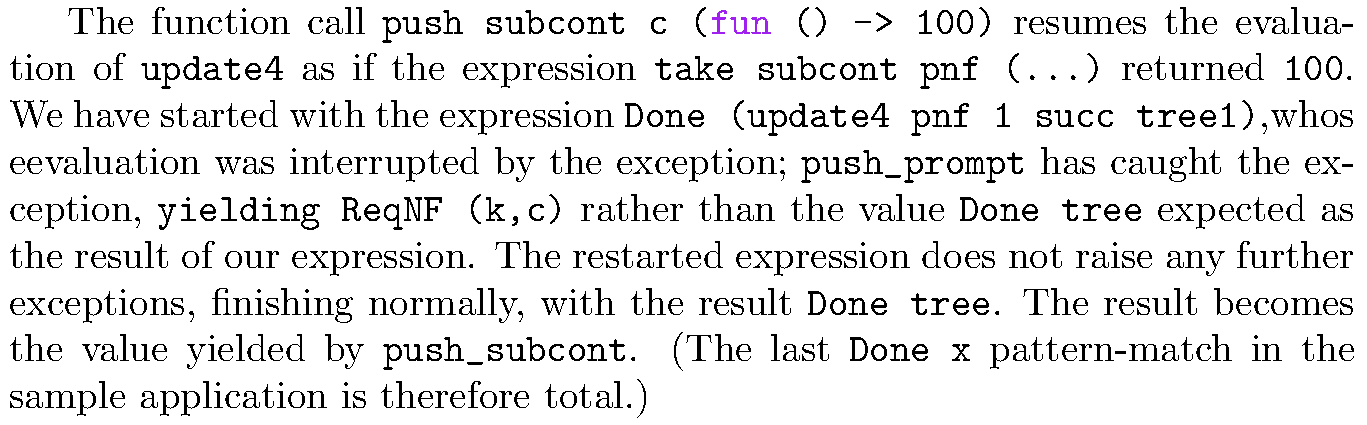
\includegraphics[width=\textwidth,height=0.8\textheight,keepaspectratio]{pipelinefigures/CodeSamplesDelimCCExplanationII.pdf}
      \end{center}      
    \end{figure}
  \end{frame}
  \begin{frame}
    \frametitle{in-place update with delimcc}    
    \begin{figure}[ht]
      \begin{center}        
        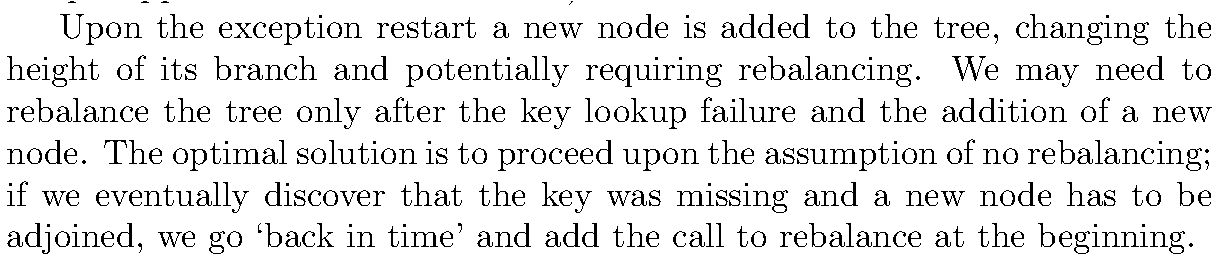
\includegraphics[width=\textwidth,height=0.8\textheight,keepaspectratio]{pipelinefigures/CodeSamplesDelimCCExplanationIII.pdf}
      \end{center}      
    \end{figure}
  \end{frame}
%   \begin{frame}
%     \frametitle{in-place update with delimcc}    
%     \begin{figure}[ht]
%       \begin{center}        
%         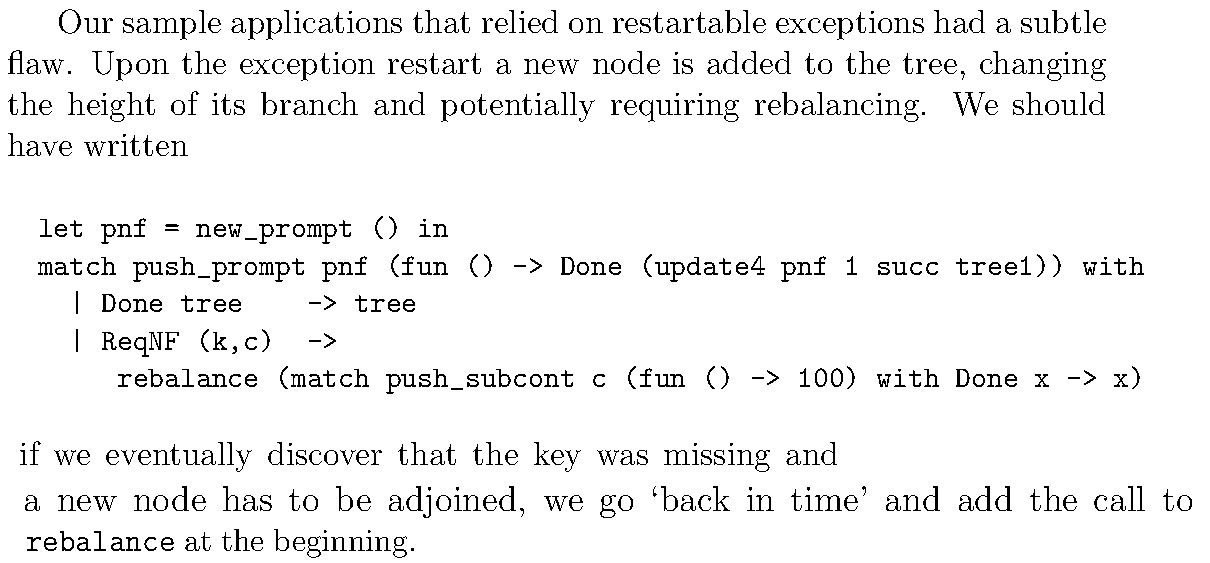
\includegraphics[width=\textwidth,height=0.7\textheight,keepaspectratio]{pipelinefigures/InplaceUpdateElaboration.pdf}
%       \end{center}      
%     \end{figure}
%   \end{frame}
  \subsection{More realistic examples: concurrency}
  \begin{frame}
    \frametitle{concurrency}    
    \begin{figure}[ht]
      \begin{center}        
        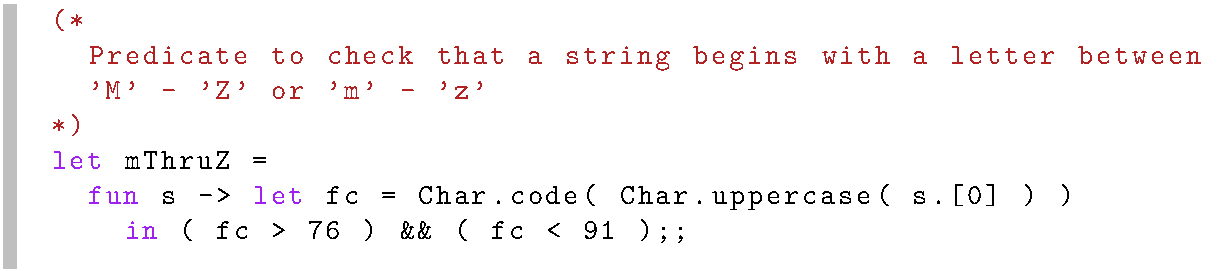
\includegraphics[width=\textwidth,height=0.7\textheight,keepaspectratio]{pipelinefigures/CodeSamplesConcurrencyHelpPredicate.pdf}
      \end{center}      
    \end{figure}    
  \end{frame}
  \begin{frame}
    \frametitle{concurrency}    
    \begin{figure}[ht]
      \begin{center}        
        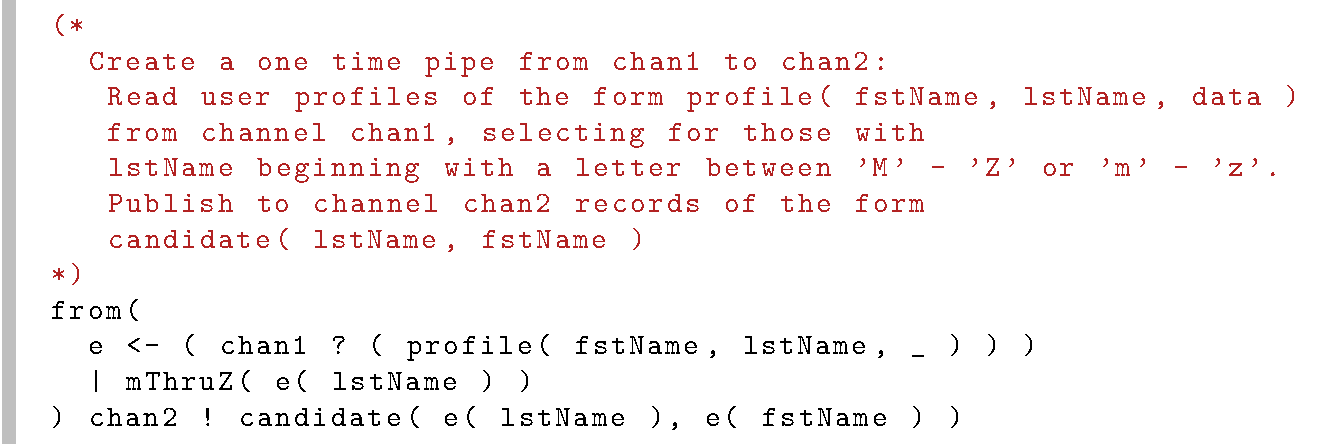
\includegraphics[width=\textwidth,height=0.7\textheight,keepaspectratio]{pipelinefigures/CodeSamplesOneTimePipe.pdf}
      \end{center}      
    \end{figure}
  \end{frame}
  \begin{frame}
    \frametitle{concurrency}    
    \begin{figure}[ht]
      \begin{center}        
        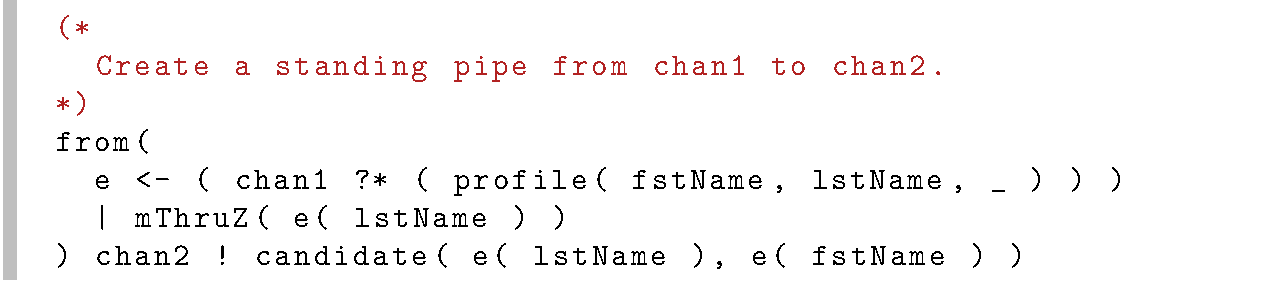
\includegraphics[width=\textwidth,height=0.7\textheight,keepaspectratio]{pipelinefigures/CodeSamplesStandingPipe.pdf}
      \end{center}      
    \end{figure}
  \end{frame}
  \begin{frame}
    \frametitle{concurrency}    
    \begin{figure}[ht]
      \begin{center}        
        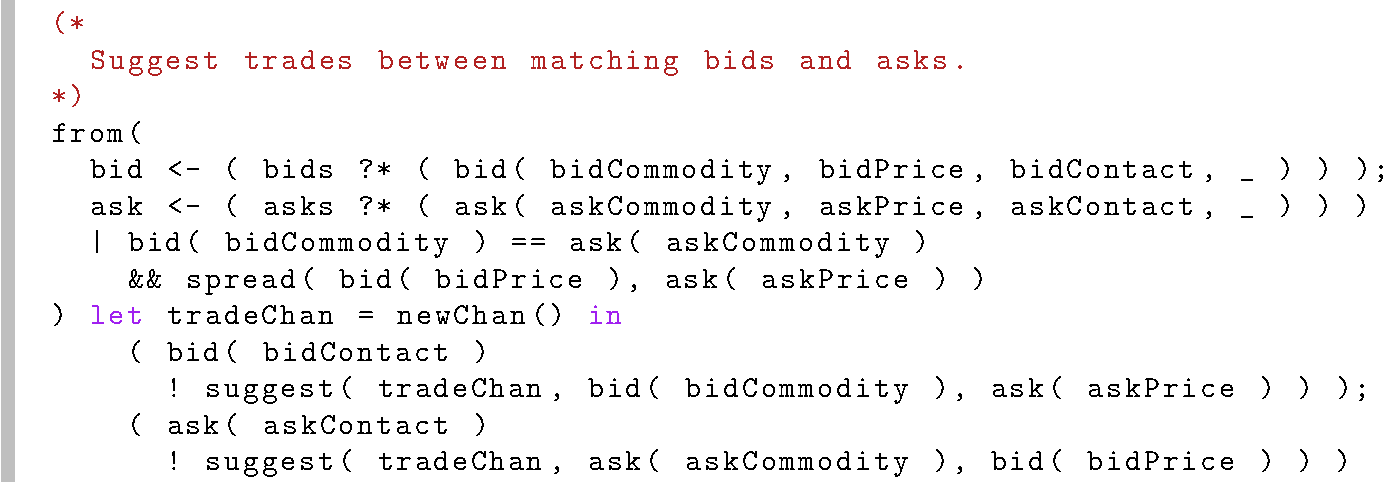
\includegraphics[width=\textwidth,height=0.7\textheight,keepaspectratio]{pipelinefigures/CodeSamplesMatchingBidsToAsks.pdf}
      \end{center}      
    \end{figure}
  \end{frame}
  \section{The pipeline}
  \begin{frame}
    \frametitle{The pipeline}
    \begin{figure}[ht]
      \begin{center}        
        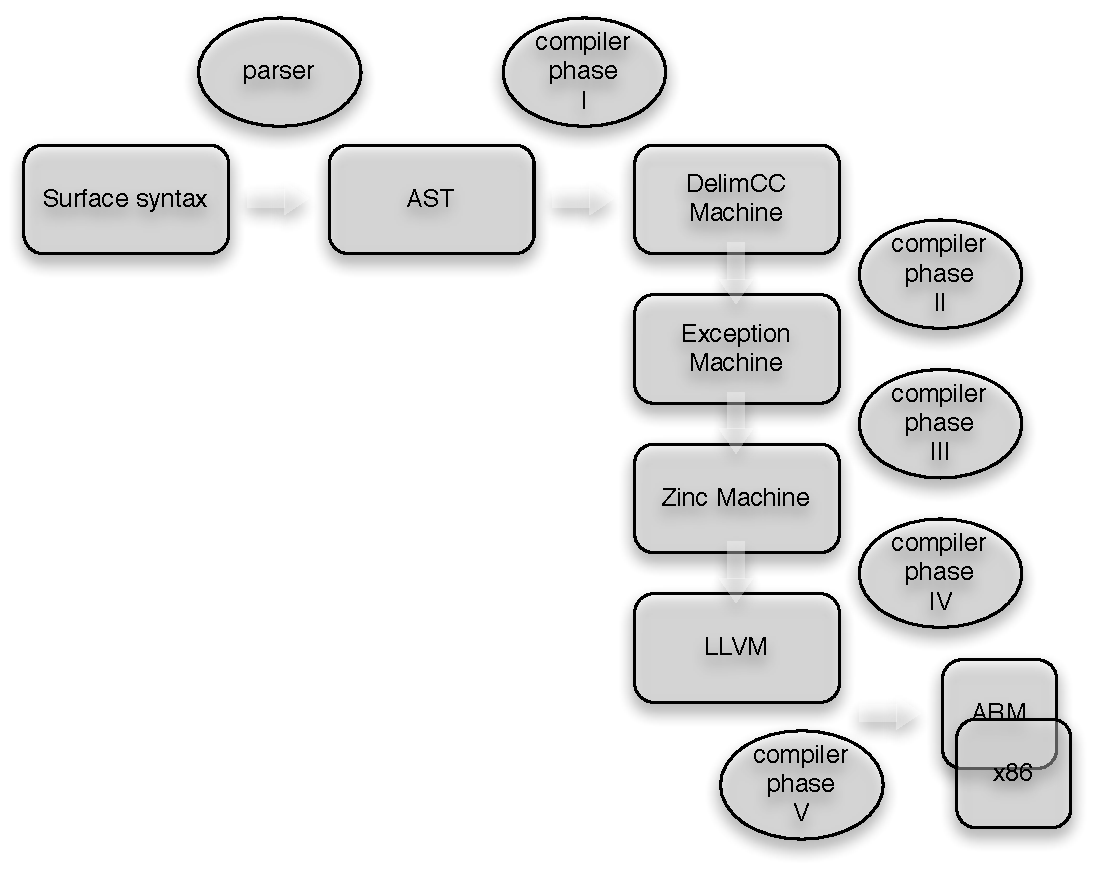
\includegraphics[height=2in]{pipelinefigures/PipelineImageI.pdf}
      \end{center}      
    \end{figure}
  \end{frame}
  \section{The delimCC machine}
  \begin{frame}
    \frametitle{The delimCC machine}
    \begin{figure}[ht]
      \begin{center}        
        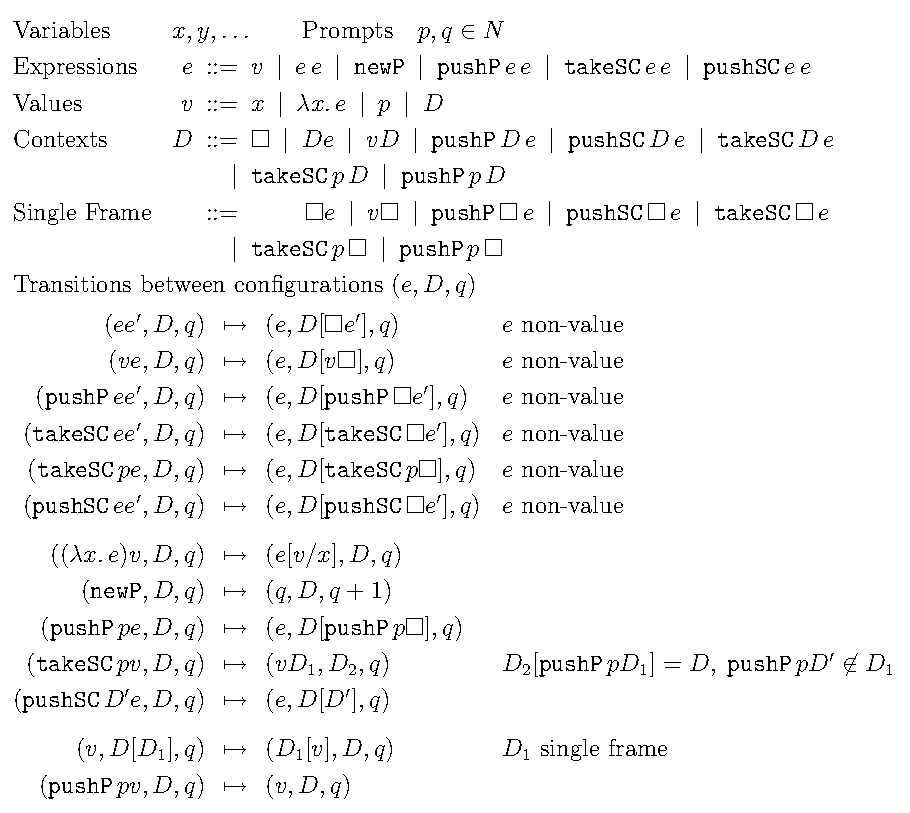
\includegraphics[height=2in]{pipelinefigures/DelimCCMachineSpecI.pdf}
      \end{center}      
    \end{figure}

  \end{frame}
  \section{The exception machine}
  \begin{frame}
    \frametitle{The exception machine}
    \begin{figure}[ht]
      \begin{center}        
        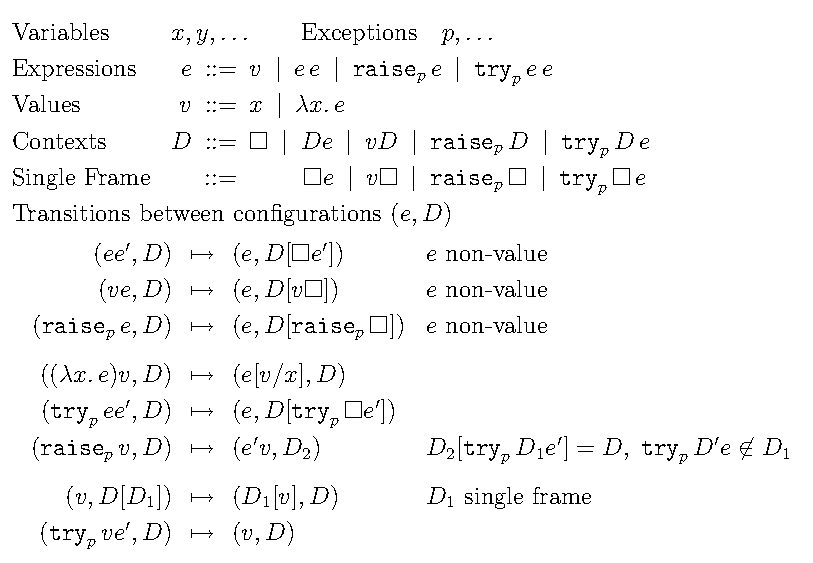
\includegraphics[height=2in]{pipelinefigures/ExceptionMachineSpecI.pdf}
      \end{center}      
    \end{figure}
  \end{frame}
  \section{Eliminating the middle men}
  \begin{frame}
    \frametitle{Eliminating the middle men}
    \begin{figure}[ht]
      \begin{center}        
        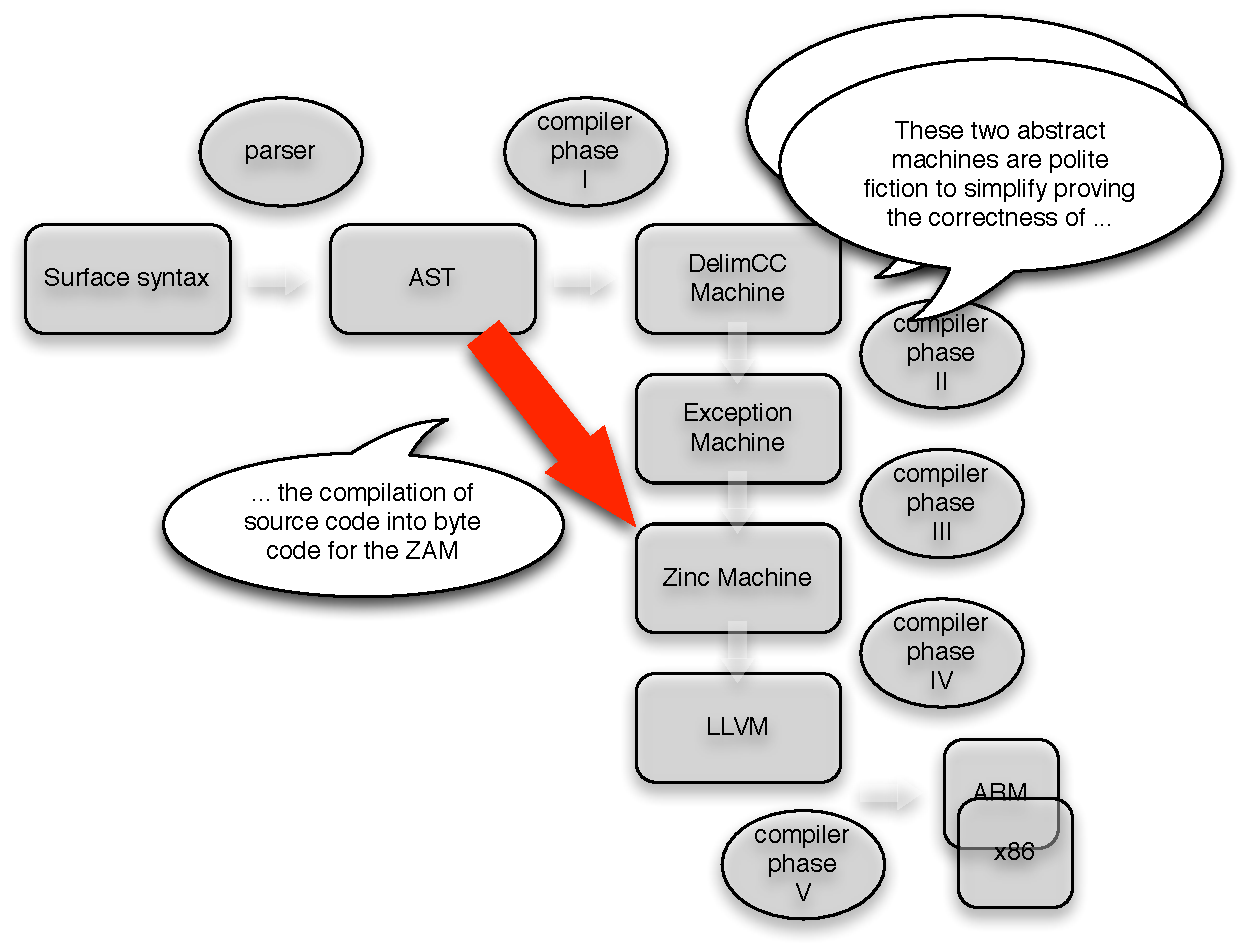
\includegraphics[height=2in]{pipelinefigures/PoliteFictions.pdf}
      \end{center}      
    \end{figure}

  \end{frame}
  \begin{frame}
    \frametitle{Eliminating the delimCC machine}
    \begin{figure}[ht]
      \begin{center}        
        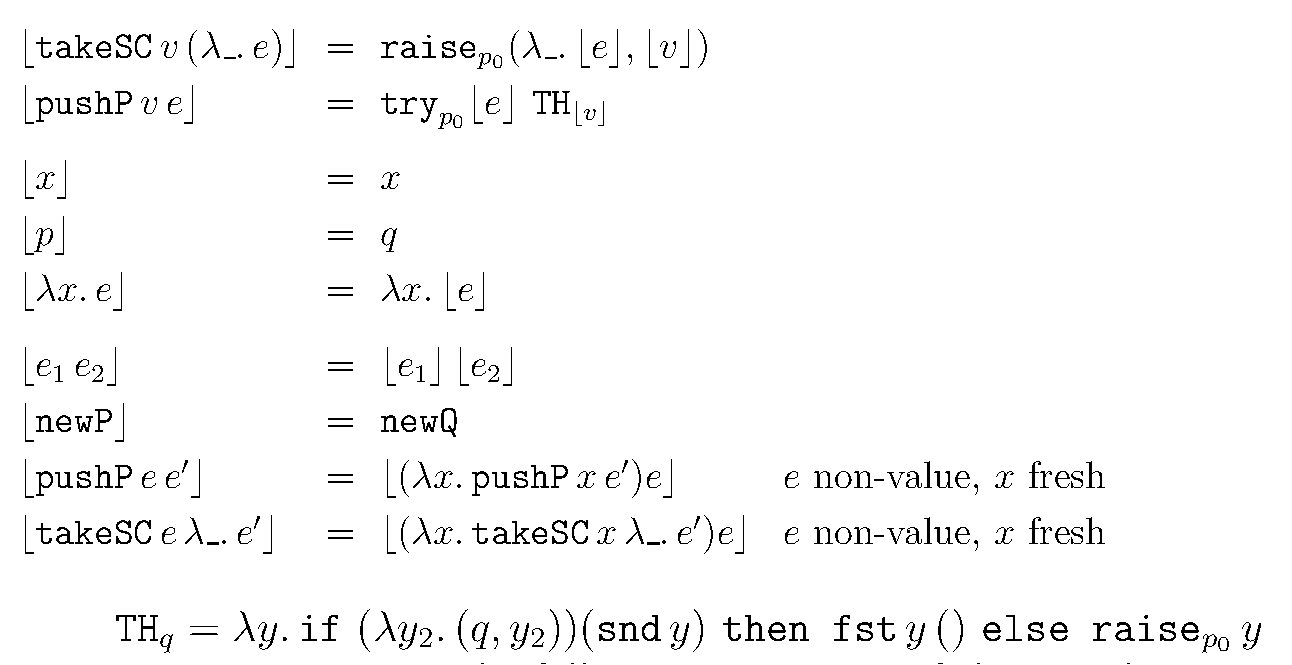
\includegraphics[height=2in]{pipelinefigures/EliminatingDelimCCMachine.pdf}
      \end{center}      
    \end{figure}

  \end{frame}
  \begin{frame}
    \frametitle{Eliminating the Exception machine} The Exception
    machine is really only a simplification of the the Zinc
    machine. It embeds directly into the Zinc machine. It's sole
    purpose is to provide an abstract target for the elimination of
    delimited continuation sugar to any abstract machine that supports
    exceptions such as the Zinc machine or the JVM or ...
  \end{frame}
  \begin{frame}
    \frametitle{Eliminating the Exception machine} 
    Thus, of our examples, only those that incur a dependency on
    \begin{figure}[ht]
      \begin{center}        
        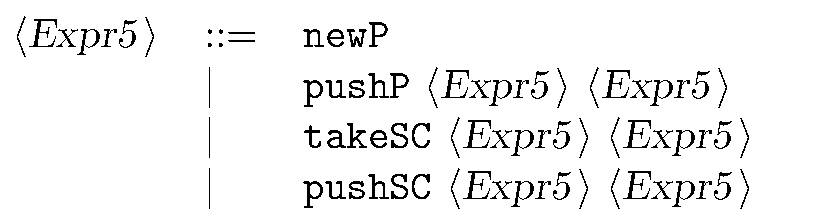
\includegraphics[width=\textwidth,height=0.3\textheight,keepaspectratio]{pipelinefigures/SyntaxSugarDelimCC.pdf}
      \end{center}      
    \end{figure}
    will have a different compilation path.
  \end{frame}
  \begin{frame}
    \frametitle{Eliminating the middle men}    
    In symbols, suppose
$C : OCamlSource \rightarrow ZincByteCode$, and $\ldb - \rdb$ is the
desugaring map from above then our compiler,
$CS : CacaoScriptSource \rightarrow ZincByteCode$
is just the composition of $C \circ \ldb - \rdb$ $ = C(\ldb - \rdb)$.
  \end{frame}
  \begin{frame}
    \frametitle{Eliminating the Exception machine} 
    To illustrate the point:
    \begin{figure}[ht]
      \begin{center}        
        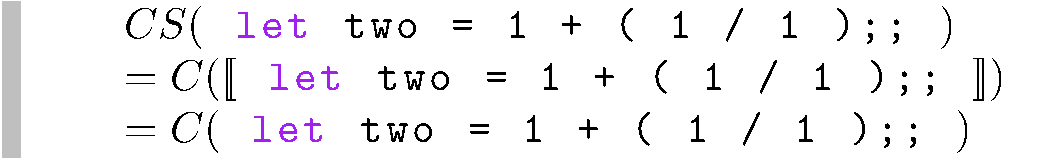
\includegraphics[width=\textwidth,height=0.2\textheight,keepaspectratio]{pipelinefigures/CompilationPathwayCore.pdf}
      \end{center}      
    \end{figure}
    
  \end{frame}
  \section{The Zinc machine}
  \begin{frame}
    \frametitle{The Zinc machine}
    This is well documented.
    
  \end{frame}
  \begin{frame}
    \frametitle{Compiling our examples to the Zinc machine}
    \begin{figure}[ht]
      \begin{center}        
        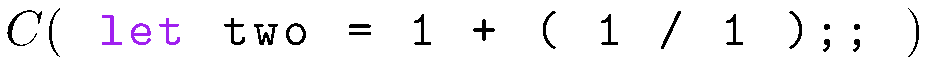
\includegraphics[width=\textwidth,height=0.075\textheight,keepaspectratio]{pipelinefigures/CompilerPathwayArithmeticExampleCompilationInvocation.pdf}
      \end{center}      
    \end{figure}        
    \begin{figure}[ht]
      \begin{center}        
        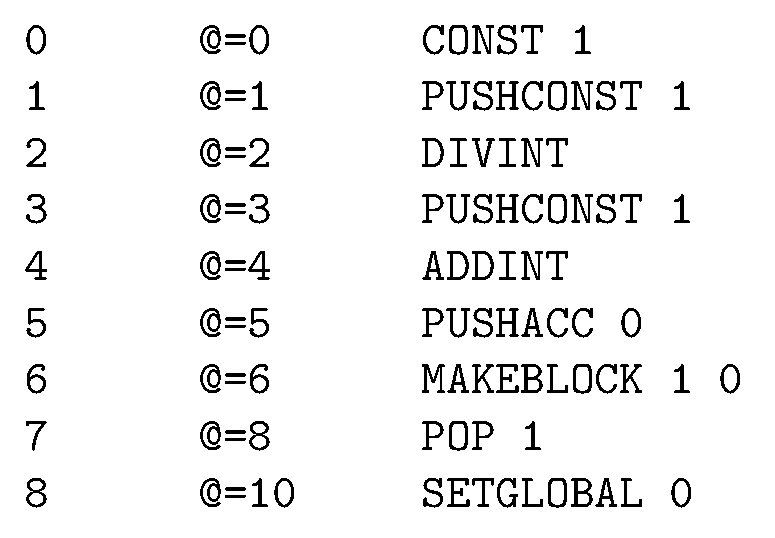
\includegraphics[width=\textwidth,height=0.6\textheight,keepaspectratio]{pipelinefigures/CompilationPathwayArithmeticExampleBytecode.pdf}
      \end{center}      
    \end{figure}        
  \end{frame}
  \begin{frame}
    \frametitle{Compiling our examples to the Zinc machine}
    \begin{figure}[ht]
      \begin{center}        
        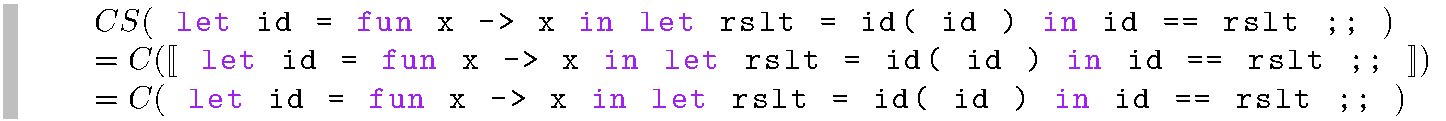
\includegraphics[width=\textwidth,height=0.15\textheight,keepaspectratio]{pipelinefigures/CompilerPathwayCoreLanguageAbstractionApplication.pdf}
      \end{center}      
    \end{figure}        
    \begin{figure}[ht]
      \begin{center}        
        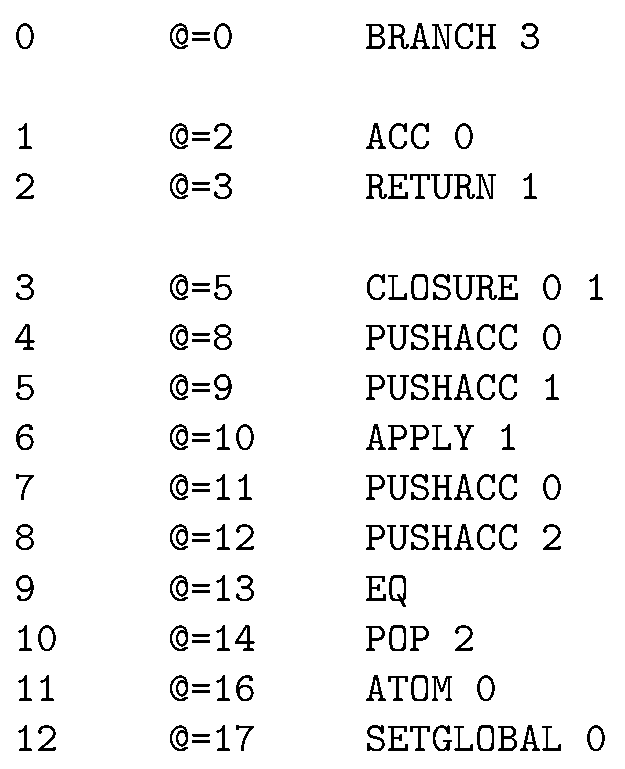
\includegraphics[width=\textwidth,height=0.52\textheight,keepaspectratio]{pipelinefigures/CompilerPathwayCoreLanguageAbsAppByteCode.pdf}
      \end{center}      
    \end{figure}        
  \end{frame}
  \section{LLVM}
  \begin{frame}
    \frametitle{The LLVM} The purpose of targeting LLVM from the Zinc
    machine byte code (the subject of various student projects in the
    OCaml community) is to be able to target a variety of hardware
    architectures, notably the mobile platforms.
  \end{frame}
  \section{Conclusions}
  \begin{frame}
    \frametitle{Conclusions}
  \end{frame}
\end{document}